% Partie 1.2 - Les différents protocoles et topologies %

\subsection{Les différents protocoles et topologies}

\subsubsection{Les différentes topologies}

Un réseau local (\textbf{LAN} pour \textit{Local Area Network}) est un réseau où les terminaux peuvent communiquer sans avoir besoin d'un accès Internet. Mais il existe un autre type de réseau plus proche de nos contraintes, le réseau personnel (\textbf{PAN} pour \textit{Personal Area Network)}. Dans ce type de réseau le but est de faire aboutir les échanges entre les divers éléments du réseau avec des puissances assez faible pour garantir une autonomie correcte. Ce qui correspond bien à nos besoins avec les capteurs. Ils ont besoins d'être autonome le plus longtemps possible tout en évitant une interaction humaine physique direct. 

Dans le monde des réseau, nous utilisons le terme topologie pour définir l'arrangement des différents nœuds dans un réseau. Avec les réseaux PAN, on se limite assez souvent à deux topologies: maillage partielle (\textbf{mesh}) et en étoile (\textbf{star}).

La topologie en étoile est extrêmement rependue car c'est celle qui est utilisée dans le modèle maître-esclave(s). Le maître est le point névralgique du réseau, toutes les communications sont obligées de passer par lui. Cela se révèle assez pratique dans le cas de la collecte de données car le maître est le point de convergence en plus d'être le point de sortie du réseau.

Cette topologie est en parfaite opposition au maillage partielle. En effet dans cette dernière topologie chaque nœuds est potentiellement un routeur, et chaque routeur un potentiel point de sortie. Ces routeur sont appelés des \textit{Edge Router} ou \textit{Border Router}, ils font le lien entre le PAN et d'autres réseaux. Les End Devices ne routent pas l'information.

\begin{figure}[h]
\begin{center}
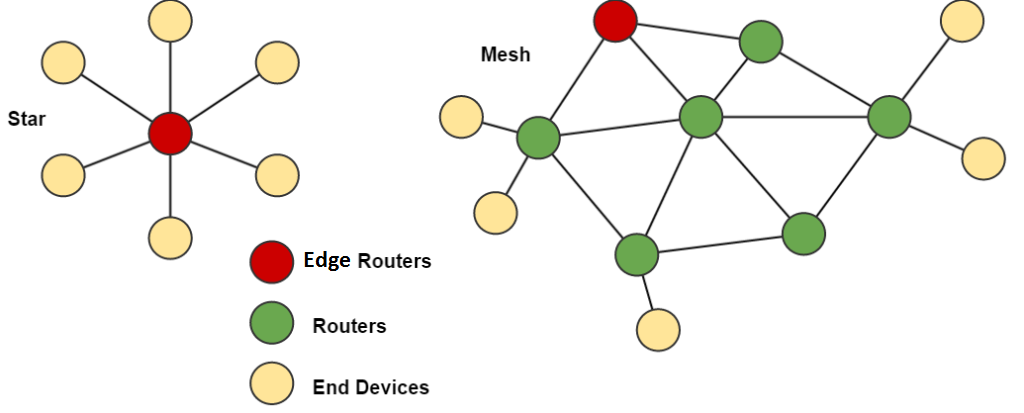
\includegraphics[width=15cm]{\rpDossier/images/topologies.png}
\end{center}
\caption{Topologies}
\label{topologies}
\end{figure}

Le fait est que comme cette technologie est explorée par plusieurs constructeur et organisme, plusieurs protocoles ont vu le jour, mais sans réel standard, chacun utilise celui qu'il veut. Cela pose pas mal de problème avec l'interopérabilité des éléments dans le réseau qui est pourtant une des caractéristiques phare de l'IoT. Voici une liste succincte de ces divers protocoles.

\subsubsection{les différents protocoles}

Dans cette partie nous allons vous présenter divers protocoles orientés basse consommation. Ces protocoles sont développées par divers organismes ce qui fait qu'aucun n'est un standard, les constructeurs implémentent ceux qui veulent. Cela peut poser certains problèmes d'interopérabilités, et augmenter fortement le prix des appareils.

\textbf{Bluetooth} : protocole sans-fil opérant dans la bande 2.4 GHz. Il a été conçue pour l'échange de données sur de courtes distances mais ne tenait pas bien compte de la consommation. Généralement, un dongle USB permettait l'ajout du bluetooth à son PC mais la technologies est devenue tellement commune qu'elle est maintenant complètement intégrée dans l'hardware de nos équipements. Bluetooth utilise exclusivement une topologies en étoiles ce qui n'est pas très pratique pour l'établissement de grand réseau (en terme de nombre et de surface).

Bluetooth IoT

\textbf{Wi-Fi} :

\textbf{Zigbee} : ce protocole repose sur les couches basses définis par \textbf{802.15.4} (aussi utilisé par 6LoWPAN et défini dans la partie suivante). Il supporte des topologies en étoiles et maillées (\textit{mesh}), mais pour cela, un des équipements doit avoir le rôle de "coordinateur". Le coordinateur est généralement l'appareil avec le plus de puissance et il est la racine du réseau, il peut avoir plusieurs rôles comme faire la liaison entre réseaux ou bien un aire de stockage pour les clés de sécurités. Il ne peut y avoir qu'un seul coordinateur par réseau et dans le cas d'un réseau en étoile il est forcément au centre.

La technologie utilisant ce protocole est conçue comme une alternative plus simple et moins chère que celles des autres WPANs, comme Bluetooth ou Wi-Fi. La portée varie beaucoup en fonction de la bande de fréquence utilisé mais à titre d'exemple, la portée à 2.4 GHz en intérieur varie en 10 et 20 mètres. Les débits sont aussi relativement faible: 20 kbit/s si l'on opère dans la bande 868 MHz et 250 kbit/s à 2.4 GHz. Les faibles débits permettent de maintenir une consommation extrêmement faible, ce qui fait en sorte que les équipements tiennent plusieurs années.

\textbf{Z-Wave} :

\textbf{IrDA} :